% !TEX root = ../main.tex
\newpage
\section{Hebbian Learning and Synaptic Plasticity} \label{sec:HebbianLearningAndSynapticPlasticity}
\vspace{1mm}
\begin{quote}
\textsl{When an axon of cell A is near enough to excite a cell B and repeatedly or persistently takes part in firing it, some growth process or metabolic change takes places in one or both cells such that A's efficiency, as one of the cells firing B, is increased.}\cite{Hebb1949}
\end{quote}

This quote from Hebb has influenced the neuroscientific community since 1949. In its essence, Hebb postulated that neurons that \textsl{fire together, wire together}. It has since become known as \textsl{Hebbian learning}, and is simply modelled as a positive correlation between the action potentials of spiking neurons. It has been proven in vivo in many studies \cite{ChrolCannon2014}, just like its counterpart, \textsl{anti-Hebbian learning}, where a negative correlation can be found.


\subsection{Spike-timing dependant plasticity}
One specific temporal interpretation of these ideas is \textsl{spike-timing-dependent plasticity} (\STDP), where the relative timing of action potentials from the pre- and postsynaptic neuron determine causality \cite{Kempter1999, Gerstner2002}. If the postsynaptic neuron fires right after the presynaptic neuron, then we can expect the synaptic strength from post- to presynaptic neuron to increase, and vice versa. 

Let us say that neuron $\theta_i$ spikes at time $t_i$ and that neuron $\theta_j$ spikes at $t_j$. Taking the time difference $\Delta t_{ij}$ as $t_j - t_i$, we can say that when $\Delta t_{ij} > 0$ the spikes are correlated (there exists a temporally causal relation), and we can model an increase in synaptic strength of the connection from $\theta_i$ to $\theta_j$, which we will gather in the \textsl{coupling matrix} $K_{ij}$. In the same fashion we can decrease $K_{ji}$ when $\Delta t_{ij} < 0$ as there is no causal relation. 

We will find an expression for $\Delta K_{ij}$ in function of $\Delta t_{ij}$ so that at each time-step we can update $K_{ij} \leftarrow K_{ij} + \Delta K_{ij}$.\\

We can think of the coupling matrix as the continuous interpretation of $\kappa A_{ij}$, where synaptic strength and network topology go hand in hand. This also means that we need to redefine some concepts:
\begin{align}
\kinbi = \sum_{j=1}^{N} \rvert K_{i j} \rvert \hspace{15mm} 
\koutbj = \sum_{i=1}^{N} \rvert K_{i j} \rvert \hspace{15mm} 
\kmean &= \frac{1}{N} \sum_{i,j=1}^{N} \rvert K_{i j} \rvert \hspace{15mm}  \label{eq:redefineFromK}  %\hat{\kmean} = \frac{1}{N} \sum_{i,j=1}^{N} K_{i j}
\end{align}
The absolute value ensures that we capture the magnitude of the coupling strength. The reason we want to distinguish between $\kmean$ and $\hat{\kmean}$ is that for some parts of the investigation it is beneficial to study how inhibitive and excitatory coupling strengths influence each other.\\

The functions $W(t)$ that relate $\Delta t_{ij}$ to $\Delta K_{ij}$ are called \textsl{learning windows},  as they define a range in which $K_{ij}$ is able to adapt or \textsl{learn}, and also when learning is optimal. When signals between neurons show a very large time difference (negative or positive) we do not expect them to be correlated. Because the learning windows are generally not symmetrical we can also expect the coupling matrix to be asymmetrical.

Another characteristic is the integral over the learning window. A window with a negative integral directs synaptic strengths mostly towards inhibitory behaviour, and vice versa with a positive integral. An integral of zero would mean that both inhibitory and excitatory synapses are stimulated equally. It has been proven that $\int W(\tau) \mathop{d\tau}$ is the magnitude of the correlation between signals \cite{Gerstner2002}. \\

%The magnitude of change is modulated by an asymmetric biphasic learning window around pulses originating from the postsynaptic neuron. Asymmetric because the peak is not situated at 0 and the integral over the window is generally positive, biphasic because this allows both to strengthen and weaken coupling strengths \cite{Gerstner2002}. 

This approach simplifies modeling the neuronal back-propagation, where another pulse is generated as an echo of the action potential which travels through the neuron dendrites (so, backwards). This behavior is believed to adjust the presynaptic weights, though it is a controversial subject \cite{Gerstner2002}. 


\subsection{Formulations of \STDP as a model}
Following the notation in \cite{Kempter1999}, we will denote the sequence of action potentials, the \textsl{spike train}, coming from each neuron $\theta_i$ as $S_i^{\rm out}(t) = \sum_{n} \delta (t-t_{i}^{n})$, where $t_{i}^{n}$ is the time that $\theta_i$ has fired. Similarly, we will denote the spike train coming into each neuron $\theta_i$ as $S_i^{\rm in}(t) = \sum_{f} \delta (t-t_{i}^{f})$ with $t_{i}^{f}$ being the time that a neighbouring neuron has spiked. Now we can say that the synaptic strengths are adjusted as:
\begin{align}
\Delta K_{ij} &= \int_{t}^{t+\mathcal{T}} w^{\rm{out}} S_i^{\rm out}(\tau) + w^{\rm{in}} S_{j}^{\rm {in}}(\tau) \mathrm{d}\tau
+ \iint_{t}^{t+\mathcal{T}} W( \tau^\prime - \tau) S_{i}^{\rm out}(\tau) S_{j}^{\rm in}( \tau^\prime) \mathrm{d} \tau \mathrm{d} \tau^\prime
\label{eq:KempterSTDPFormulation1} \\
&= \sum_{t_i^{n}\in \mathcal{T}} w^{\mathrm{out}} + \sum_{t_{j}^{f} \in \mathcal{T}} w^{\mathrm{in}} + \sum_{t_{j}^{f}, \: t_i^{n} \in \mathcal{T}} \hspace{-2mm} W (t_{j}^{f}-t_i^{n} ) \label{eq:KempterSTDPFormulation2}
\end{align}
with $\mathcal{T}$ the period over which learning occurs. $w^{\mathrm{in}} > 0$ and $w^{\mathrm{out}} < 0$ are small weights on the in- and outgoing action potentials. These can be used to counteract the inhibitive or excitatory nature of the results of $W$ and are necessary for $K_{ij}$ to reach an equilibrium. This is proven from the average learning dynamics, \cite{Kempter1999}. In \eqref{eq:KempterSTDPFormulation1} we can recognise the correlation between signals as a convolution over the learning window. \\

The following learning window is proposed:
\begin{align}
W(t)_K = A
\begin{cases}
\left[\left(1-\frac{t}{\tilde{\tau}_{p}}\right) - \left(1-\frac{t}{\tilde{\tau}_{n}}\right)\right] \cdot \exp \left( \frac{t}{\tau_{\rm syn}} \right) & \text{for } t \leq 0 \\
 \exp \left(-\frac{t}{\tau_{p}}\right) - \exp \left(-\frac{t}{\tau_{n}} \right) & \text{for } t > 0
\end{cases} \label{eq:learningwindowKempter1999}
\end{align}
Here $t$ is the delay between presynaptic spike arrival and postsynaptic firing, $A$ is a small learning parameter and all $\tau$ are time constants. The values are given as $A = 10^{-5}$, $\tau_{\rm syn} = 5$ ms, $\tau_{p} = 1$ ms and $\tau_{n} = 20$ ms. $\tilde{\tau}_{p} \equiv \tau_{\rm syn} \tau_{p} / (\tau_{\rm syn} + \tau_{p})$ and $\tilde{\tau}_{n} \equiv \tau_{\rm syn} \tau_{n} / (\tau_{\rm syn} + \tau_{n})$. $\int W(\tau)_K \mathop{d \tau} = 4.75 \times 10^{-8}$ so that the correlation is positive. \\

To counteract the excitatory nature of the learning window, the authors propose $w^{\mathrm{in}} = A$ and $w^{\mathrm{out}} = -1.0475A$ so that the amplitude of these weights is on the same order as the magnitude of the learning window \cite{Kempter1999}. This is a regulatory process, as neurons are punished for sending out  many spikes over time by decreasing their influence over neighbours more than the increase in influence of their neighbours over them. This threshold can be overcome by teaching the neurons to spike at the right time (with respect to its neighbours' spikes) as then the learning window yields an increase in synaptic strength. This process is inherently asymmetric. \\

Using different processes to generate spike trains, the learning equation \eqref{eq:KempterSTDPFormulation2} converges to a stable equilibrium \cite{Kempter1999}. The question will now be whether that is still the case when we will apply \STDP to our network of Theta neurons, as changes to the coupling strength will also influence the spiking dynamics between neurons, which in turn will affect the learning again.\\

Another formulation of \STDP as a mathematical model can be found in \cite{Song2000}. It is postulated without being concerned about the biological aspect too much, simplifying some of the ideas of \cite{Kempter1999}. The synaptic strengths are simply updated with:
\begin{align}
\Delta K_{ij} &= K^{\rm max} \cdot \sum_{t_{j}^{f}, \: t_i^{n} \in \mathcal{T}} \hspace{-2mm} W (t_{j}^{f}-t_i^{n} ) \label{eq:SongSTDPFormulation}
\end{align}
where $K^{\rm max}$ is the maximum allowed synaptic strength, so that we can think of \eqref{eq:SongSTDPFormulation} as taking a percentage of the maximum coupling. The authors also constrain $0 \leq K_{ij} \leq K^{\rm max}$, as there is no regulatory process like in \eqref{eq:KempterSTDPFormulation2}. In their further work on \STDP and \IP the authors booked remarkable progress, and their work is very interesting for our application \cite{Song2017}. 

The learning window is then again defined as a discontinuous function:
\begin{align}
W(t)_S =
\begin{cases}
A_{n} \cdot \exp \left(\frac{t}{\tau_n}\right)  & \text{for } s \leq 0 \\
A_{p} \cdot \exp \left(\frac{-t}{\tau_p}\right) & \text{for } s > 0 
\end{cases} \label{eq:learningwindowSong2000}
\end{align}
where we will use $A_p = 0.005$, $A_n = -0.00525$ and $\tau_p = \tau_n = 20$ ms. $\int W(\tau)_S \mathop{d \tau} = -5.0 \times 10^{-6}$ so we expect the weights to be suppressed towards a negative value. Interestingly, the line between reward and punishment is very thin, as the largest increase and largest decrease in synaptic strength lie right next to each other on the spectrum. \\

Recently, triphasic learning windows have been used to account for when it takes too long for the postsynaptic neuron to fire, and thus to decorrelate the relation between neurons. These learning windows are curves that were fitted to experimental data of the cortex and the hippocampus \cite{ChrolCannon2014}. 
Extending the work of \cite{Song2000} we can find a brief investigation of network topology and clustering using triphasic windows, \cite{ChrolCannon2012}. The method is as in \eqref{eq:learningwindowSong2000}, with the following learning window:
\begin{align}
W(t)_C = A_{p} \cdot \exp \left(\frac{-\left(t - 15 \right)^{2}}{ \tau_{p}}\right) - A_{n} \cdot \exp \left(\frac{-\left(t - 20\right)^{2}}{ \tau_{n}}\right)  \label{eq:learningwindowChrolCannon2012}
\end{align}
where $A_{p}=0.23$, $A_{n}=0.15$, $\tau_{p}=200$ and $\tau_n = 2000$. $\int W(s)_C \mathrm{d}s = -6.0 \times 10^{-3}$. \\

When comparing the qualities of the different learning windows presented here, one can quickly notice the difference in magnitude between the learning windows. That does not necessarily include the magnitude of the correlation, but the magnitude of the window itself. In \eqref{eq:learningwindowKempter1999}, the learning rate is a few orders of magnitude smaller than in \eqref{eq:learningwindowChrolCannon2012} and this resulted in extremely slow convergence when testing. For \eqref{eq:learningwindowSong2000} this issue was solved in \cite{ChrolCannon2012} by using $A _p = 0.1$ and $A_n = -0.12$. In the same spirit, we will therefore use $A = 8.0 \times 10^{-2}$ in \eqref{eq:learningwindowKempter1999}. These alterations yield $\int W(\tau)_S \mathop{d \tau} = -4.0 \times 10^{-4}$ and $\int W(\tau)_K \mathop{d \tau} = 3.8 \times 10^{-4}$.

\begin{figure}[H]
\centering
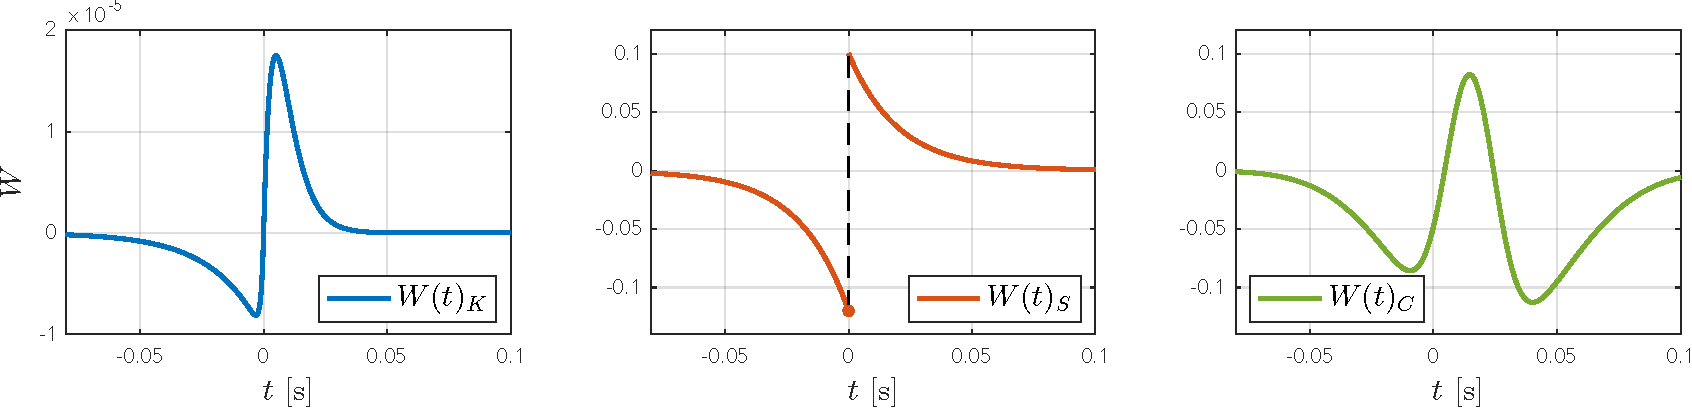
\includegraphics[width = \textwidth]{../Figures/Learning/LearningWindows.pdf}
\caption{Three different biphasic learning windows. Left: with $W_K$ the the learning spectrum is quite narrow. Middle: we can see how in $W(t)_s$ a slightly larger emphasis is put on the anti-Hebbian learning. Right: a triphasic window can punish the synaptic strength when signals arrive either too early or too late.}
\label{fig:LearningWindows}
\end{figure}

%The learning windows generally have $W(t^{\ast}) = 0$ for $t^{\ast} \geq 0$. This means that no learning will take place when the delay between neuron spikes is exactly $t^{\ast} \geq 0$. The triphasic windows show two of those points. 

It is important to notice that learning only occurs when neurons spike, so that equilibrium states will disturb the learning process. However, these states were rarely encountered during the testing process, and it seems like there continues to exist enough randomness in the states of $\theta_i$ to persist spiking.
When implementing \STDP, a time-step smaller than 0.01 is necessary, otherwise important details in the learning dynamics that are captured by the shape of the learning window will be lost. \\

In recent years, criticism on \STDP has been growing, as experimental data has shown that \STDP is usually accompanied by homeostatic plasticity of the neurons excitability and the synaptic strength. Basing our learning behaviour on the correlation between neuronal activity can be quite unstable: changes to the synaptic strength cause changes in the postsynaptic firing rate, which generates further changes to the synaptic strength in a positive feedback loop. Processes like \textsl{intrinsic plasticity} (\IP), where one neuron's excitability changes over time as to self-regulate sensitivity to incoming action potentials, or \textsl{synaptic scaling}, where synapse characteristics are adjusted in unison to counteract positive feedback loops, have proven to stabilise the synchronisation \cite{ChrolCannon2014, Kirkwood2019}. When \STDP and \IP are combined, it seems like the two process balance each other out and stable network topologies can be found \cite{Song2017}.
%We can model intrinsic plasticity by adjusting the neuron's excitability as the inverse of the firing rate: he more spikes that a neuron will receive, the less affected it is \cite{Song2017}.  An observed phenomenon is that the excitability evolves together with the coupling strength, but that at the extremes this relation reverses \cite{Debanne2017, Debanne2018}.  These types of plasticities should be relatively easy to implement but have no impact on the network topology.


\subsection{Synaptic scaling}
There is no upper or lower bound on the synapse strength, and generally connection strengths are nonzero. Positive reinforcement loops might disturb the learning process, which would not be beneficial for the model. One technique we can apply to keep the strengths within a definitive range is to scale homeostatically - a method where any increases in synaptic strength will balance out any decreases by scaling:
\begin{align}
K_{ij}^s = K_{ij} \frac{\frac{1}{N} \sum_{i,j} K_{ij}}{\sum_{i} K_{ij}}
\end{align}
In this way, the out-degrees will remain constant. Using this approach, something has to remain constant, whether that is $\kmean$, or $\kmean^2$ or any other property of the adjacency matrix. However, this property is not what we are after: we want a method that is able to change the network topology entirely.


\subsection{Intrinsic plasticity}
Instead of scaling the weights to preserve a certain quantity in the network, we can allow the neurons to adjust their sensitivity to incoming signals. So when some synaptic strengths are increased, we can reduce the excitability, and vice-versa. This should counteract positive feedback. In \cite{Song2017} such a method is introduced in detail. We can simply update $\eta_{i} \leftarrow \eta_{i} + \eta_{\max } \cdot \phi_{i}$, where: 
\begin{minipage}{.45\textwidth}
   \centering
   \begin{figure}[H]
	\centering
	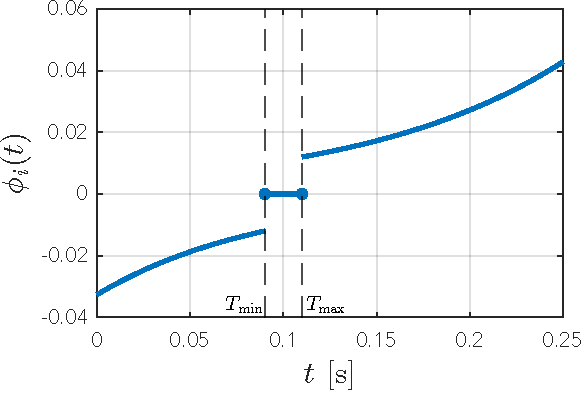
\includegraphics[width = \textwidth]{../Figures/Learning/IPlearningFunction.pdf}
	%\caption{The learning behaviour for intrinsic plasticity as proposed in \cite{Song2017}.}
	\label{fig:IPlearningFunction}
	\end{figure}
\end{minipage}
\begin{minipage}{.55\textwidth}
\begin{align}
	\phi_{i} (t) =
	\begin{cases}
	-\alpha \cdot \exp \left(\frac{T_{\min }-t}{T_{\rm min }}\right) \hspace{10mm} t<T_{ \rm min } \\ 
	\alpha \cdot \exp \left(\frac{t-T_{\rm max }}{T_{\max }}\right) \hspace{12mm} t >T_{\rm max } \\ 
	0 \hspace{24.5mm} T_{ \rm min } \leq t \leq T_{\rm max }
	\end{cases}
\end{align}
\vspace{10mm}
\end{minipage}
The argument $t$ represents the time that has passed between successive spike of the same neuron, the \textsl{inter-spike interval} (\ISI). This is always a positive number.

%\begin{figure}[H]
%\centering
%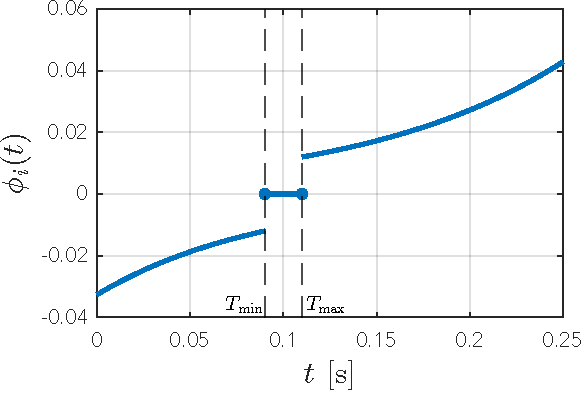
\includegraphics[width = 0.5\textwidth]{../Figures/Learning/IPlearningFunction.pdf}
%\caption{The learning behaviour for intrinsic plasticity as proposed in \cite{Song2017}.}
%\label{fig:IPlearningFunction}
%\end{figure}

%\textcolor{red}{QUESTION}: \textsl{is it necessary to include more background theory on Hebbian Learning?}
